% !TEX root = dissertationmain.tex
%Chapter
\chapter{Introduction}
\label{chap:chapter1}

\paragraph{}This section will give a brief background and history of Machine Learning before going in to depth with the definitions and types of algorithms used in modern Machine Learning systems. An analyses of the impact Machine Learning has in the field of computer security and how it can be applied directly to penetration testing and red teaming. Research aims and objectives will be provided as well as a statement to the structure of the rest entire thesis.

%Section
\section{Background}
\label{sec:section1}

\paragraph{}The term machine learning was first defined by Arthur Samuel in the year 1959 as a "Field of study that gives computers the ability to learn without being explicitly programmed" and later as "a field of study that concentrates on induction algorithms and on other algorithms that can be said to 'learn'", \cite{ronKohavi}. Machine learning has largely evolved from several subfields of artificial intelligence, specifically, computational learning and pattern recognition but now it stands on its own with its subfield Deep Learning being at the forefront of technology. Machine learning consists of the studying and construction of algorithms that can learn from and make predictions of data, \cite{bigData}. The early information available for machine learning was almost entirely theoretical due to the lack of processing power at the time. One of the early pioneers was \cite{Valiant} whom developed a PAC learning framework and established the theory of a learnable algorithm, \cite{mlOpt}.  Modern machine learning algorithms use many calculations from statistics, information theory, theory of algorithms, probability and functional analyses, \cite{mlOpt}.

%Section
\section{Current State of Machine Learning}
\label{sec:section2}

\paragraph{}In the recent year’s, machine learning accuracy and efficiency has increased dramatically which has caused the field to rapidly gain in popularity, especially in deep learning. One of the major reasons for this is due to the improvement in graphics processing units which in some computational tasks can outperform central processing units by an order of magnitude or more, \cite{CNNperf}. The rapidly growing field of deep learning could be made apparent by Google’s recent self-driving car and LeNet image recognition system, however, examples of machine learning can be found in just about every field with a classification or regression problem. Some of which include: natural language processing using morphological analyses for linguistics (\cite{NLP}), document classification and spam detection, better image recognition than humans (\cite{manualclassifying}) and beating a professional player at the complex Chinese game ‘Go’ (\cite{Gobot}). Figure ~\ref{fig:aitimeline} illustrates the advancement of machine learning using the context of game artificial intelligence players.

%Figure
\begin{figure} 
   \centering
   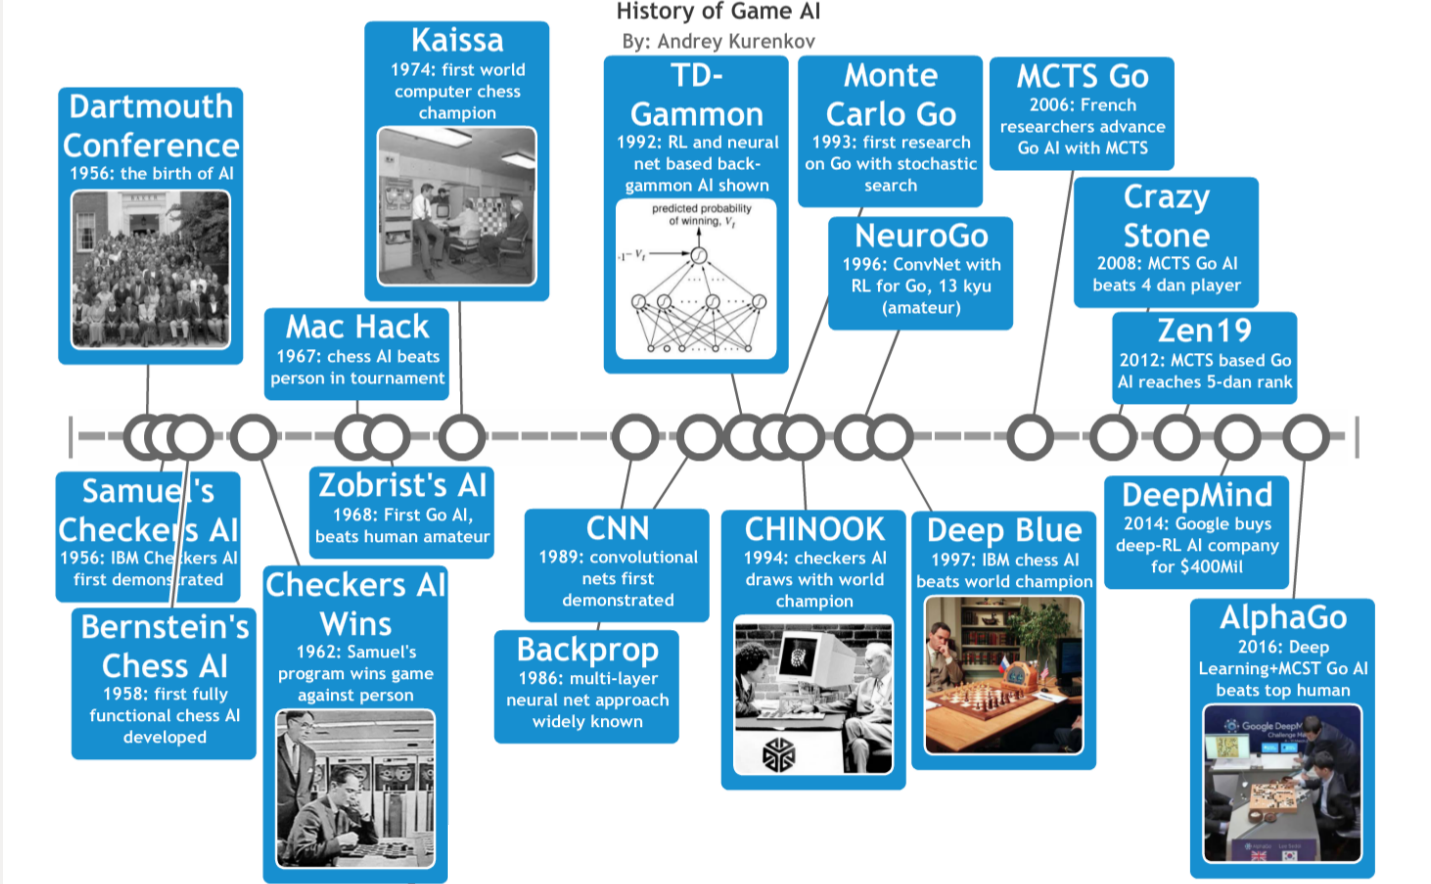
\includegraphics[width=0.95\textwidth]{Figures/aitimeline.png}
   \caption[Timeline of artificial intelligence for games]{ Timeline of artificial intelligence for games, ~\cite{timeline}}
   \label{fig:aitimeline}
\end{figure}


\paragraph{}The majority of projects over the past few years have focused on Deep Learning due to its performance and versatility with complex problems but also because of the media coverage with large scale projects by international corporations such as Google and Microsoft. The idea of deep learning has been around since the 1980’s where a Japanese scientist, Kunihiko Fukushima, proposed a hierarchical, multi-layered artificial neural network named Neocognitron, designed for handwritten character recognition. Neocognitron was recognised as the inspiration for convolutional neural networks, the most commonly used deep learning algorithm, \cite{DeepLearning}.  Deep learning attempts to model complex abstractions in data by using a multiple-level architecture most commonly compromising of artificial neural networks and non-linear transformations in its algorithms, \cite{CNNperf}.  As such, the concepts of deep learning are extensions of regular machine learning algorithms.
\paragraph{}In the past year a new topic has become of consider interest in the machine learning field, Automated Machine Learning, which can be considered to cover the tasks of algorithm selection, hyperparameter tuning, iterative modelling and model assessment, \cite{autoML}. By the end of 2016 the python Auto-sklearn library was created based off of the scikit-learn library which encompasses these tasks, created by a team from the University of Freiburg it won the KDnuggets AutoML challenge, \cite{auto-skl}. Using these examples, it’s possible to hypothesize that the future of machine learning will include automatic deep learning, however, these individual fields of machine learning are still in their infancy and far from being used together.
\paragraph{}The computer security industry due to its nature, has many examples of machine learning implementations such as intrusion detection systems using machine learning or deep learning for anomaly detection. One of which has been commercialised under the company name ‘Deep Instinct’ and advertises zero-day detection using deep learning. However, the majority are very similar and are all blue team based security solutions. Researching into Red team or penetration testing tools using machine learning resulted in a disappointing lack of tools or ideas considering the vast amount available for Blue team. 
\paragraph{}The sole documented research found for red team was for an automatic penetration testing project named Auto Red Team (ART) framework by Lu, Song of Iowa State University in 2008 which used decision trees and hard programmed exploits. This meant the entire hard programmed exploit section had to be reconstructed for each use case, this would not be ideal but also extremely time consuming. Further analyses of the ART framework can be found in the literature review of "Auto Red Team: a network attack automation framework based on decision tree". There have also been tools and libraries created to test the security of software which use machine learning models such as Deep Pwning. Deep Pwning is an open source metasploit plugin which allows the tricking of machine learning models. This field of research was named Adversarial Machine learning and the first paper of which was respectably named "Adversarial Machine Learning" and published by ACM in 2011.
\paragraph{}There is an extensive amount branches to machine learning and unfortunately, too many to cover in this thesis due to time constraints. Therefore, this introduction will only detail the most popular types of machines learning algorithms.


%Section
\section{Significance of study}
\label{sec:section3}

\paragraph{}The increased demand for penetration testers justifies the need for more effective and advanced tools to conduct their security assessments. The goal of a penetration test being to find vulnerabilities in a system using techniques similar to that of a malicious hacker. This means malicious hackers will continue to use the most advanced methods to gain access to critical systems and thus security teams must also continue to advance their toolset to be as effective and efficient as possible. Penetration tests can last a time scale of anything between one day to several months and more advanced machine learning tools would allow for a more efficient use of this time. The large variety of machine learning models used in the blue team results in a large variety of models required to test them using adversarial machine learning as well as advanced machine learning tools, specifically for the red team in order to bring each team to the same level. Having both red team and blue team on the same level is beneficial for the industry as a whole, providing competition between both sides and to continue to strive for improvement.

This project aims to help correct this unbalance by designing and developing a proof of concept red team tool using machine learning techniques.

The application must be able to be used as an aid to a security professional during a security assessment or capture the flag hacking events in order to be classed as a red teaming tool.

This application must also be scalable and versatile to be used in varying sized network environments.

The tool will be critically analysed and recommendations of related future work will be provided.

%Section
\section{Types of Machine learning}
\label{sec:section4}

\paragraph{}As mentioned above there are many different machine learning algorithms available. Each algorithm can be classed based on the problem, required output and several factors of the data set, such as whether it includes labels and the amount of values it includes. The two primary problems machine learning algorithms provide solutions to, can be put in to two categories which are not mutually exclusive and can be combined in certain use cases. These are classification and regression problems. The following describes and states the differences of these types.

\subsection{Classification} 
\label{ssec:subsection1}

\paragraph{}With the growth of big data, unstructured data is more prevalent than its structured counterpart. This is because, "while the amount of structured data has grown fast, the amount of unstructured data has grown much faster" \cite{bigData}. This creates the need for ever more efficient data analytics and is a typical classification problem for machine learning. There are many types of classification, simple types such as a linear classifier and then more complex types such as multiclass and structured classifiers. Classification is largely used in data mining and statistical analyses for these purposes. In short, classification is used when you require an input variable to be identified as part of a group or label, resulting in the full dataset being categorised. Classification can only take a finite set of values such as picking from 1 of N values. In classification, each incorrect answer is equally incorrect, compared to regression where incorrect answer can be varying levels of incorrect.

\subsection{Regression} 
\label{ssec:subsection2}

\paragraph{}Regression problems are for when prediction of real continuous values is required, such as predicting stock market values and detecting the age of a person from a picture, \cite{pythonML}. Regression analyses involves predicting and estimating a response based on previous data and input variables. As mentioned above regression answers can have a varying level of inaccuracy as appose to binary correct or false predictions. This is due to regression using continuous values.
Figure ~\ref{fig:regvsclass}  provides a basic illustration example of these two problems.

%Figure
\begin{figure} 
   \centering
   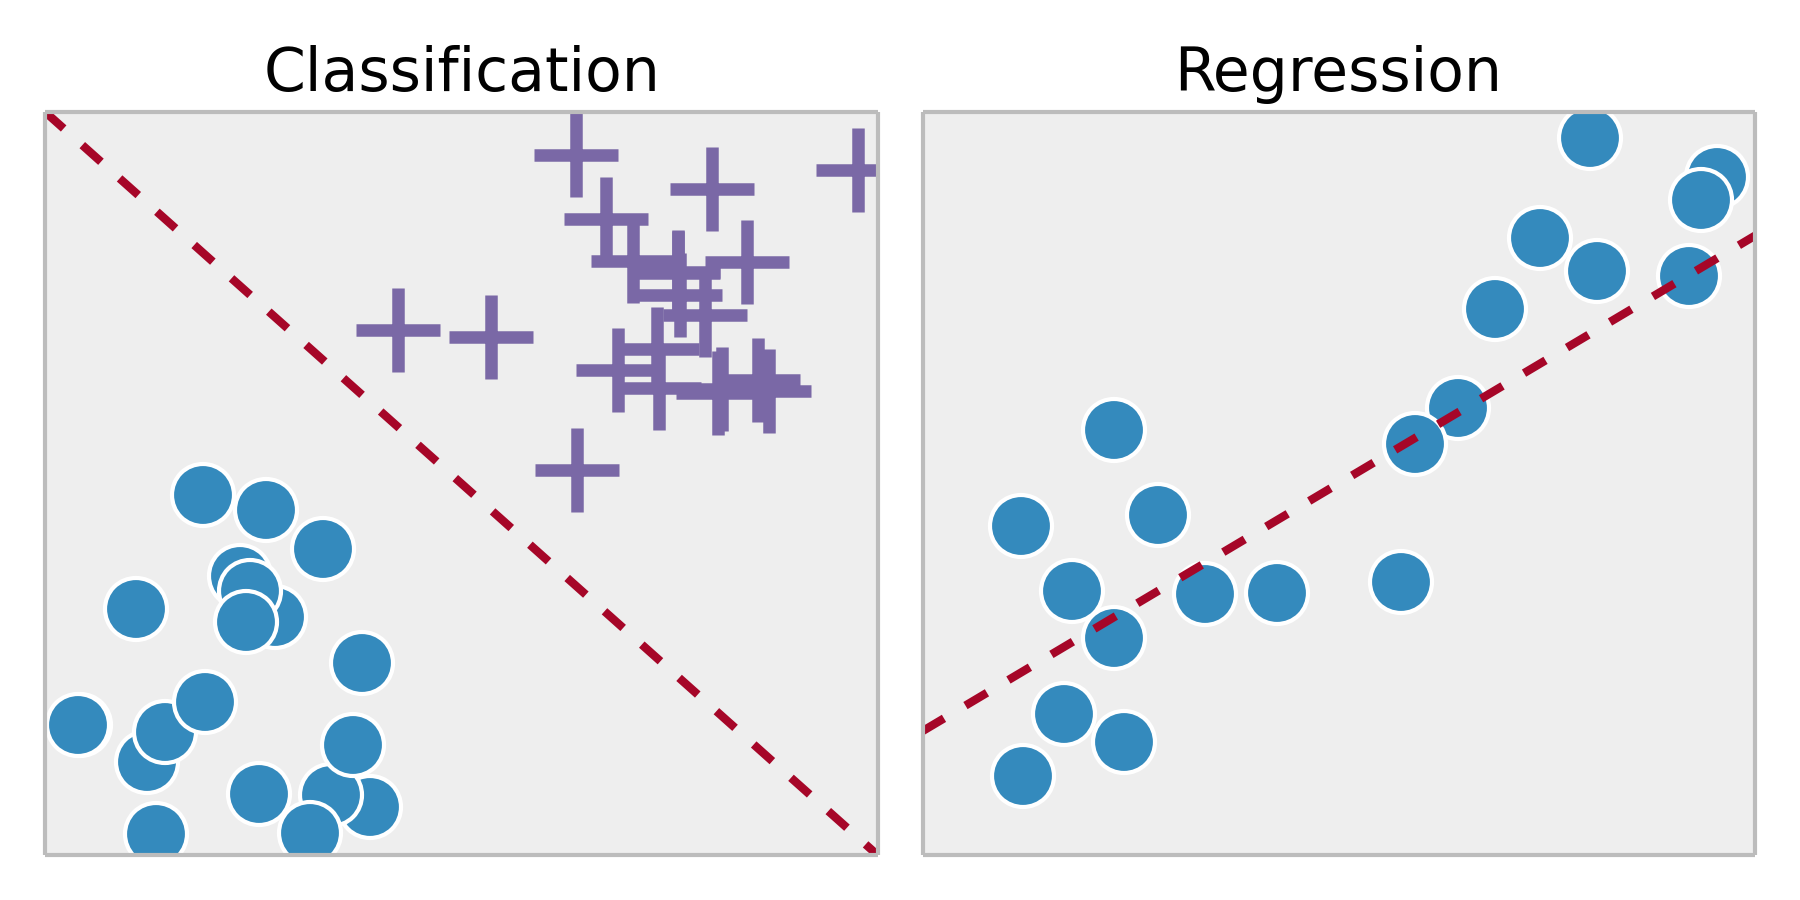
\includegraphics[width=0.95\textwidth]{Figures/ml.png}
   \caption[Illustration of machine learning types]{ Illustration of machine learning types, ~\cite{pythonML}}
   \label{fig:regvsclass}
\end{figure}


%Section
\section{Types of Learning algorithms}
\label{sec:section5}

\paragraph{}The most commonly found learning methods for algorithms are supervised and unsupervised followed by semi supervised and reinforcement learning which are also fairy common. These are explained briefly as follows.

\subsection{Supervised}
\label{ssec:subsection3}

\paragraph{}In a supervised training model, the entire data-set used for training is pre-labelled so that the algorithm can use pattern analyses to predict given values after training. A use case scenario for supervised learning includes the above stock market example where current values with labels are given and the model is used to predict future labels.

\subsection{Semisupervised} 
\label{ssec:subsection4}

\paragraph{}Due to the expensive nature of labelled data in most cases, semisupervised learning uses a split of labelled and unlabelled data to train the model. This is most often split unevenly with the large majority of training data being unlabelled. This model is often used in cases where the cost of labelled data-sets is simply too expensive.

\subsection{Unsupervised} 
\label{ssec:subsection5}

\paragraph{}The opposite of supervised learning, where the training data-set has no labels and the model must attempt to determine the correct answer itself. This is often used as a method to determine a structure in the data given. These models can identify segments of similar attributes such as clustering. Unsupervised learning is the primary method used for this thesis’s methodology.

\subsection{Reinforcement} 
\label{ssec:subsection6}
\paragraph{}Reinforcement learning works similarly to heuristic algorithms in the sense that every possibility is attempted and assigned a score in which the iteration with the highest score is used as the model output. Whilst training this model the algorithm uses the highest score’s iteration to modify its calculations for greater accuracy and efficiency. This model is often used in robotics as well as game design for path navigation calculation and computer player AI (artificial intelligence). The following is an example use case: A chess player AI calculates each possible move it can make using a reinforcement model for each of its turns. The model assigns a score to each move it could possible make at that point in time and weights them based on pieces acquired, future strategy prospects and defence risk.
Similar models have been used for AI’s mentioned in Figure ~\ref{fig:aitimeline}.


%Section
\section{Common Machine Learning Algorithms}
\label{sec:section6}

\paragraph{}As mentioned above, due to the amount of machine learning algorithms available and project time constraints, only a few of the most common algorithms will be described below.
\subsection{Linear Regression} 
\paragraph{}Linear regression predicts real values based off continuous data of two variables. It does this by using a best fit or regression line over the existing data extending in predictions. If the data does not indicate any positive or negative trends then using linear regression will likely not be a very useful model. The trend or direction of data can be calculated using correlation coefficient as follows, where $\left( {{x_2},{y_1}} \right),\left( {{x_n},{y_n}} \right)$ is the observed data.
\begin{align*}
r = \frac{1}{{n - 1}}\Sigma \left( {\frac{{x - \bar x}}{{{s_x}}}} \right)\left( {\frac{{y - \bar y}}{{{s_y}}}} \right)
\end{align*}
A value that is close to 1 would indicate positive correlation where -1 would indicate negative correlation. A normalised covariance calculation may also be used instead.
\subsection{K-Nearest Neighbours}
\label{KNN}
\paragraph{}K-nearest neighbours (or KNN) is a widely used computationally expensive supervised learning model for data classification but can also be used for regression problems. The value ‘k’ refers to the distance is which to weigh the number of class nodes inside. Several distance functions can be used such as Euclidean, Manhattan and Minkowski with the most common being Euclidean. Euclidian distance is the straight-line distance between the two nodes. On a two-dimensional plane it is measured using the following formula where the coordinates are 
${\bf{p}}{\rm{\;}} = {\rm{\;}}\left( {p1,{\rm{\;}}p2} \right){\rm{\;and\;}}{\bf{q}}{\rm{\;}} = {\rm{\;}}\left( {q1,{\rm{\;}}q2} \right)$.
\begin{align*}
d\left( {p,1} \right) = \sqrt {{{\left( {{q_1} - {p_1}} \right)}^2} + {{\left( {{q_2} - {p_2}} \right)}^2}} \;\;
\end{align*}
For e.g. if k = 1 then the current node will be assigned to the same class as its nearest node, where as if k = 5 then the class with the largest number of nodes in a distance of 5 will be selected to represent the current node. KNN is not resistant to bias in data-sets and thus data must be normalised before inputted into the model. KNN models are not to be confused with K-means clustering models as they share a very loose relationship being that KNN can be used to add data into pre-existing K-means clusters known as a nearest centroid classifier.
\subsection{K-means Clustering} 
\paragraph{}K-means Clustering is an unsupervised model in which the number of clusters is specified in advance. ‘K’ being the number of clusters the model will output for the given data. The value for K can be assigned manually or the optimal value can be calculated by using either the elbow method or the gap statistic, the latter of which is used and explained in the methodology section of this thesis with a practical use of K-means. The K-means algorithm itself is also known as Lloyd's algorithm and uses iterative refinement to determine the best clustering.
\subsection{Dimensionality Reduction} 
\label{pca}
\paragraph{}Dimensionality reduction algorithms are exactly what the name suggests. With the dramatic increase in variable types and raw data size being captured leading to the invention of the term Big Data, datasets have become very large. These large datasets have become the main bottleneck for machine learning performance, especially in computationally expensive models such as KNN’s and K-means. There needs to be a way to identify the significance of each variable in the data-set in order to give weights to their values for use in calculations. Principle Component Analyses (PCA) can be used for this purpose as well as for variance maximization. The PCA algorithm attempts to detect correlation between each of these variable types and uses this information to detect the vector directions of maximum variance in high-dimensional data. The algorithm then projects these maximum variance vectors into a smaller dimension whilst attempting to keep the most amount of information and greatest variance as possible. If the measurement scales of the dataset variables are not equal, then the data should be normalised prior to PCA due to the variance maximization functions of the algorithm.
\subsection{Decision Trees} 
\paragraph{}Decision trees are a classification model that uses supervised learning to calculate either categorical or continuous dependent variables. Decision trees can also be designed manually as was traditionally done. As the name suggests, the model works by splitting the data at each branch of the tree by asking questions and making decisions on each layer. The concept of decision trees is simple however they can be combined together, or include other machine learning models within its layers greatly increasing the complexity of this model. 
\subsection{Random Forests} 
\paragraph{}Random decision forest is one of these complications where the model contains several decision trees built during the training stage and can also be used with unsupervised learning. These random decision forests can be used for classification or regression by simply using the mode of the results from the forest or the mean in the case of a prediction problem. They creation of this model differs from regular decision trees as the training algorithm applies bootstrap aggregating, commonly referred to as bagging, followed by feature bagging resulting in a random decision forest. Bagging increases the stability and accuracy of decision trees by reducing variance and avoiding the overfitting of data. It does this by generating additional sets data based on the given data-set which results in a larger data-set overall reducing the variance but increasing the predictivity of the model. Bagging can also be used on several other machine learning algorithms. Feature bagging also known as the random subspace method, selects random samples from the entire dataset in order to reduce the correlation between each tree in the forest. This is done to produce varied models for each tree as appose to them being very similar if they were all trained on the entire data-set. Random forests can be complicated once more by adding a neural network within its layers, or even a deep learning model such as recurrent neural networks.
\subsection{Ariticial Neural Networks} 
\paragraph{}Artificial neural networks (or ANN’s) are commonly used as the bases for most deep learning algorithms such as convolutional and recurrent networks and are loosely based on the way a human brain functions. They can be used with several types of learning methods. Neural networks consist of interconnected neurons on a layered scheme in which every neuron has a function and its output can be seen by its connected neurons to then use it in their own functions. Each neural connection has an assigned weight for its output which is calculated during the training stage of the model. The layers consist of three types, an input, an output and hidden layers sandwiched between the two. The number of hidden layers in a neural network is what defines whether it is a deep learning model or not. Models with more than one hidden layer are referred to as deep learning models. How the layers are connected and the way data travels between the layers defines the type of neural network. For e.g. a recurrent neural network allows for sequences to be used for input and output unlike convolutional which can only use fixed values for these. The Google subsidiary DeepMind uses recurrent neural networks in its algorithms to create its AlphaGo AI mentioned previously.

